\documentclass[1p]{elsarticle_modified}
%\bibliographystyle{elsarticle-num}

%\usepackage[colorlinks]{hyperref}
%\usepackage{abbrmath_seonhwa} %\Abb, \Ascr, \Acal ,\Abf, \Afrak
\usepackage{amsfonts}
\usepackage{amssymb}
\usepackage{amsmath}
\usepackage{amsthm}
\usepackage{scalefnt}
\usepackage{amsbsy}
\usepackage{kotex}
\usepackage{caption}
\usepackage{subfig}
\usepackage{color}
\usepackage{graphicx}
\usepackage{xcolor} %% white, black, red, green, blue, cyan, magenta, yellow
\usepackage{float}
\usepackage{setspace}
\usepackage{hyperref}

\usepackage{tikz}
\usetikzlibrary{arrows}

\usepackage{multirow}
\usepackage{array} % fixed length table
\usepackage{hhline}

%%%%%%%%%%%%%%%%%%%%%
\makeatletter
\renewcommand*\env@matrix[1][\arraystretch]{%
	\edef\arraystretch{#1}%
	\hskip -\arraycolsep
	\let\@ifnextchar\new@ifnextchar
	\array{*\c@MaxMatrixCols c}}
\makeatother %https://tex.stackexchange.com/questions/14071/how-can-i-increase-the-line-spacing-in-a-matrix
%%%%%%%%%%%%%%%

\usepackage[normalem]{ulem}

\newcommand{\msout}[1]{\ifmmode\text{\sout{\ensuremath{#1}}}\else\sout{#1}\fi}
%SOURCE: \msout is \stkout macro in https://tex.stackexchange.com/questions/20609/strikeout-in-math-mode

\newcommand{\cancel}[1]{
	\ifmmode
	{\color{red}\msout{#1}}
	\else
	{\color{red}\sout{#1}}
	\fi
}

\newcommand{\add}[1]{
	{\color{blue}\uwave{#1}}
}

\newcommand{\replace}[2]{
	\ifmmode
	{\color{red}\msout{#1}}{\color{blue}\uwave{#2}}
	\else
	{\color{red}\sout{#1}}{\color{blue}\uwave{#2}}
	\fi
}

\newcommand{\Sol}{\mathcal{S}} %segment
\newcommand{\D}{D} %diagram
\newcommand{\A}{\mathcal{A}} %arc


%%%%%%%%%%%%%%%%%%%%%%%%%%%%%5 test

\def\sl{\operatorname{\textup{SL}}(2,\Cbb)}
\def\psl{\operatorname{\textup{PSL}}(2,\Cbb)}
\def\quan{\mkern 1mu \triangleright \mkern 1mu}

\theoremstyle{definition}
\newtheorem{thm}{Theorem}[section]
\newtheorem{prop}[thm]{Proposition}
\newtheorem{lem}[thm]{Lemma}
\newtheorem{ques}[thm]{Question}
\newtheorem{cor}[thm]{Corollary}
\newtheorem{defn}[thm]{Definition}
\newtheorem{exam}[thm]{Example}
\newtheorem{rmk}[thm]{Remark}
\newtheorem{alg}[thm]{Algorithm}

\newcommand{\I}{\sqrt{-1}}
\begin{document}

%\begin{frontmatter}
%
%\title{Boundary parabolic representations of knots up to 8 crossings}
%
%%% Group authors per affiliation:
%\author{Yunhi Cho} 
%\address{Department of Mathematics, University of Seoul, Seoul, Korea}
%\ead{yhcho@uos.ac.kr}
%
%
%\author{Seonhwa Kim} %\fnref{s_kim}}
%\address{Center for Geometry and Physics, Institute for Basic Science, Pohang, 37673, Korea}
%\ead{ryeona17@ibs.re.kr}
%
%\author{Hyuk Kim}
%\address{Department of Mathematical Sciences, Seoul National University, Seoul 08826, Korea}
%\ead{hyukkim@snu.ac.kr}
%
%\author{Seokbeom Yoon}
%\address{Department of Mathematical Sciences, Seoul National University, Seoul, 08826,  Korea}
%\ead{sbyoon15@snu.ac.kr}
%
%\begin{abstract}
%We find all boundary parabolic representation of knots up to 8 crossings.
%
%\end{abstract}
%\begin{keyword}
%    \MSC[2010] 57M25 
%\end{keyword}
%
%\end{frontmatter}

%\linenumbers
%\tableofcontents
%
\newcommand\colored[1]{\textcolor{white}{\rule[-0.35ex]{0.8em}{1.4ex}}\kern-0.8em\color{red} #1}%
%\newcommand\colored[1]{\textcolor{white}{ #1}\kern-2.17ex	\textcolor{white}{ #1}\kern-1.81ex	\textcolor{white}{ #1}\kern-2.15ex\color{red}#1	}

{\Large $\underline{12a_{0919}~(K12a_{0919})}$}

\setlength{\tabcolsep}{10pt}
\renewcommand{\arraystretch}{1.6}
\vspace{1cm}\begin{tabular}{m{100pt}>{\centering\arraybackslash}m{274pt}}
\multirow{5}{120pt}{
	\centering
	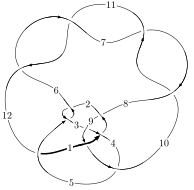
\includegraphics[width=112pt]{../../../GIT/diagram.site/Diagrams/png/1720_12a_0919.png}\\
\ \ \ A knot diagram\footnotemark}&
\allowdisplaybreaks
\textbf{Linearized knot diagam} \\
\cline{2-2}
 &
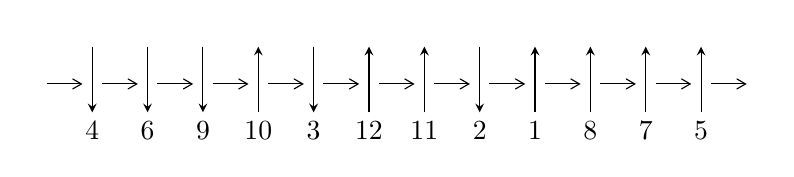
\begin{tikzpicture}[x=20pt, y=17pt]
	% nodes
	\node (C0) at (0, 0) {};
	\node (C1) at (1, 0) {};
	\node (C1U) at (1, +1) {};
	\node (C1D) at (1, -1) {4};

	\node (C2) at (2, 0) {};
	\node (C2U) at (2, +1) {};
	\node (C2D) at (2, -1) {6};

	\node (C3) at (3, 0) {};
	\node (C3U) at (3, +1) {};
	\node (C3D) at (3, -1) {9};

	\node (C4) at (4, 0) {};
	\node (C4U) at (4, +1) {};
	\node (C4D) at (4, -1) {10};

	\node (C5) at (5, 0) {};
	\node (C5U) at (5, +1) {};
	\node (C5D) at (5, -1) {3};

	\node (C6) at (6, 0) {};
	\node (C6U) at (6, +1) {};
	\node (C6D) at (6, -1) {12};

	\node (C7) at (7, 0) {};
	\node (C7U) at (7, +1) {};
	\node (C7D) at (7, -1) {11};

	\node (C8) at (8, 0) {};
	\node (C8U) at (8, +1) {};
	\node (C8D) at (8, -1) {2};

	\node (C9) at (9, 0) {};
	\node (C9U) at (9, +1) {};
	\node (C9D) at (9, -1) {1};

	\node (C10) at (10, 0) {};
	\node (C10U) at (10, +1) {};
	\node (C10D) at (10, -1) {8};

	\node (C11) at (11, 0) {};
	\node (C11U) at (11, +1) {};
	\node (C11D) at (11, -1) {7};

	\node (C12) at (12, 0) {};
	\node (C12U) at (12, +1) {};
	\node (C12D) at (12, -1) {5};
	\node (C13) at (13, 0) {};

	% arrows
	\draw[->,>={angle 60}]
	(C0) edge (C1) (C1) edge (C2) (C2) edge (C3) (C3) edge (C4) (C4) edge (C5) (C5) edge (C6) (C6) edge (C7) (C7) edge (C8) (C8) edge (C9) (C9) edge (C10) (C10) edge (C11) (C11) edge (C12) (C12) edge (C13) ;	\draw[->,>=stealth]
	(C1U) edge (C1D) (C2U) edge (C2D) (C3U) edge (C3D) (C4D) edge (C4U) (C5U) edge (C5D) (C6D) edge (C6U) (C7D) edge (C7U) (C8U) edge (C8D) (C9D) edge (C9U) (C10D) edge (C10U) (C11D) edge (C11U) (C12D) edge (C12U) ;
	\end{tikzpicture} \\
\hhline{~~} \\& 
\textbf{Solving Sequence} \\ \cline{2-2} 
 &
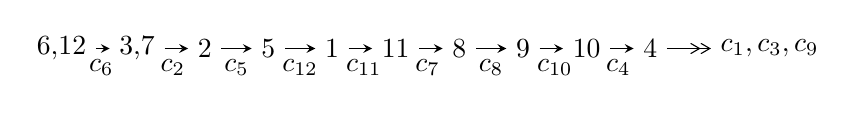
\begin{tikzpicture}[x=23pt, y=7pt]
	% node
	\node (A0) at (-1/8, 0) {6,12};
	\node (A1) at (17/16, 0) {3,7};
	\node (A2) at (17/8, 0) {2};
	\node (A3) at (25/8, 0) {5};
	\node (A4) at (33/8, 0) {1};
	\node (A5) at (41/8, 0) {11};
	\node (A6) at (49/8, 0) {8};
	\node (A7) at (57/8, 0) {9};
	\node (A8) at (65/8, 0) {10};
	\node (A9) at (73/8, 0) {4};
	\node (C1) at (1/2, -1) {$c_{6}$};
	\node (C2) at (13/8, -1) {$c_{2}$};
	\node (C3) at (21/8, -1) {$c_{5}$};
	\node (C4) at (29/8, -1) {$c_{12}$};
	\node (C5) at (37/8, -1) {$c_{11}$};
	\node (C6) at (45/8, -1) {$c_{7}$};
	\node (C7) at (53/8, -1) {$c_{8}$};
	\node (C8) at (61/8, -1) {$c_{10}$};
	\node (C9) at (69/8, -1) {$c_{4}$};
	\node (A10) at (11, 0) {$c_{1},c_{3},c_{9}$};

	% edge
	\draw[->,>=stealth]	
	(A0) edge (A1) (A1) edge (A2) (A2) edge (A3) (A3) edge (A4) (A4) edge (A5) (A5) edge (A6) (A6) edge (A7) (A7) edge (A8) (A8) edge (A9) ;
	\draw[->>,>={angle 60}]	
	(A9) edge (A10);
\end{tikzpicture} \\ 

\end{tabular} \\

\footnotetext{
The image of knot diagram is generated by the software ``\textbf{Draw programme}" developed by Andrew Bartholomew(\url{http://www.layer8.co.uk/maths/draw/index.htm\#Running-draw}), where we modified some parts for our purpose(\url{https://github.com/CATsTAILs/LinksPainter}).
}\phantom \\ \newline 
\centering \textbf{Ideals for irreducible components\footnotemark of $X_{\text{par}}$} 
 
\begin{align*}
I^u_{1}&=\langle 
-1.07123\times10^{220} u^{119}-3.52410\times10^{220} u^{118}+\cdots+4.05368\times10^{221} b+2.42001\times10^{222},\\
\phantom{I^u_{1}}&\phantom{= \langle  }2.71699\times10^{222} u^{119}+7.36929\times10^{222} u^{118}+\cdots+8.51272\times10^{222} a-2.15694\times10^{224},\\
\phantom{I^u_{1}}&\phantom{= \langle  }u^{120}+3 u^{119}+\cdots-113 u+21\rangle \\
I^u_{2}&=\langle 
- u^{23}-5 u^{22}+\cdots+b-2,\;u^{25}+4 u^{24}+\cdots+a+1,\;u^{26}+4 u^{25}+\cdots+4 u+1\rangle \\
\\
\end{align*}
\raggedright * 2 irreducible components of $\dim_{\mathbb{C}}=0$, with total 146 representations.\\
\footnotetext{All coefficients of polynomials are rational numbers. But the coefficients are sometimes approximated in decimal forms when there is not enough margin.}
\newpage
\renewcommand{\arraystretch}{1}
\centering \section*{I. $I^u_{1}= \langle -1.07\times10^{220} u^{119}-3.52\times10^{220} u^{118}+\cdots+4.05\times10^{221} b+2.42\times10^{222},\;2.72\times10^{222} u^{119}+7.37\times10^{222} u^{118}+\cdots+8.51\times10^{222} a-2.16\times10^{224},\;u^{120}+3 u^{119}+\cdots-113 u+21 \rangle$}
\flushleft \textbf{(i) Arc colorings}\\
\begin{tabular}{m{7pt} m{180pt} m{7pt} m{180pt} }
\flushright $a_{6}=$&$\begin{pmatrix}1\\0\end{pmatrix}$ \\
\flushright $a_{12}=$&$\begin{pmatrix}0\\u\end{pmatrix}$ \\
\flushright $a_{3}=$&$\begin{pmatrix}-0.319169 u^{119}-0.865680 u^{118}+\cdots-155.503 u+25.3378\\0.0264262 u^{119}+0.0869360 u^{118}+\cdots+27.3115 u-5.96992\end{pmatrix}$ \\
\flushright $a_{7}=$&$\begin{pmatrix}1\\- u^2\end{pmatrix}$ \\
\flushright $a_{2}=$&$\begin{pmatrix}-0.292742 u^{119}-0.778744 u^{118}+\cdots-128.191 u+19.3679\\0.0264262 u^{119}+0.0869360 u^{118}+\cdots+27.3115 u-5.96992\end{pmatrix}$ \\
\flushright $a_{5}=$&$\begin{pmatrix}0.320534 u^{119}+1.07174 u^{118}+\cdots+84.2977 u-8.85376\\-0.142529 u^{119}-0.544385 u^{118}+\cdots-1.27315 u+0.0747437\end{pmatrix}$ \\
\flushright $a_{1}=$&$\begin{pmatrix}0.129398 u^{119}+0.456206 u^{118}+\cdots+5.28891 u+12.2308\\0.109214 u^{119}+0.363655 u^{118}+\cdots+20.1200 u-4.71432\end{pmatrix}$ \\
\flushright $a_{11}=$&$\begin{pmatrix}- u\\u^3+u\end{pmatrix}$ \\
\flushright $a_{8}=$&$\begin{pmatrix}u^2+1\\- u^4-2 u^2\end{pmatrix}$ \\
\flushright $a_{9}=$&$\begin{pmatrix}-0.420935 u^{119}-1.00889 u^{118}+\cdots-259.731 u+36.0750\\0.0214302 u^{119}-0.0238555 u^{118}+\cdots+32.0363 u-4.61416\end{pmatrix}$ \\
\flushright $a_{10}=$&$\begin{pmatrix}- u^3-2 u\\u^5+3 u^3+u\end{pmatrix}$ \\
\flushright $a_{4}=$&$\begin{pmatrix}0.372713 u^{119}+1.18328 u^{118}+\cdots+111.600 u-12.7517\\-0.130679 u^{119}-0.522369 u^{118}+\cdots-4.64557 u+0.380200\end{pmatrix}$\\&\end{tabular}
\flushleft \textbf{(ii) Obstruction class $= -1$}\\~\\
\flushleft \textbf{(iii) Cusp Shapes $= -1.52939 u^{119}-5.38696 u^{118}+\cdots-149.423 u+4.34876$}\\~\\
\newpage\renewcommand{\arraystretch}{1}
\flushleft \textbf{(iv) u-Polynomials at the component}\newline \\
\begin{tabular}{m{50pt}|m{274pt}}
Crossings & \hspace{64pt}u-Polynomials at each crossing \\
\hline $$\begin{aligned}c_{1}\end{aligned}$$&$\begin{aligned}
&u^{120}-7 u^{119}+\cdots-7 u+3
\end{aligned}$\\
\hline $$\begin{aligned}c_{2},c_{5}\end{aligned}$$&$\begin{aligned}
&u^{120}+7 u^{119}+\cdots-6493 u+976
\end{aligned}$\\
\hline $$\begin{aligned}c_{3}\end{aligned}$$&$\begin{aligned}
&u^{120}+u^{119}+\cdots+24 u+8
\end{aligned}$\\
\hline $$\begin{aligned}c_{4}\end{aligned}$$&$\begin{aligned}
&u^{120}- u^{119}+\cdots+45 u+1
\end{aligned}$\\
\hline $$\begin{aligned}c_{6},c_{7},c_{10}\\c_{11}\end{aligned}$$&$\begin{aligned}
&u^{120}-3 u^{119}+\cdots+113 u+21
\end{aligned}$\\
\hline $$\begin{aligned}c_{8}\end{aligned}$$&$\begin{aligned}
&u^{120}- u^{119}+\cdots+4850 u+311
\end{aligned}$\\
\hline $$\begin{aligned}c_{9}\end{aligned}$$&$\begin{aligned}
&u^{120}-5 u^{119}+\cdots+3 u+8
\end{aligned}$\\
\hline $$\begin{aligned}c_{12}\end{aligned}$$&$\begin{aligned}
&u^{120}- u^{119}+\cdots+18390924 u+2188589
\end{aligned}$\\
\hline
\end{tabular}\\~\\
\newpage\renewcommand{\arraystretch}{1}
\flushleft \textbf{(v) Riley Polynomials at the component}\newline \\
\begin{tabular}{m{50pt}|m{274pt}}
Crossings & \hspace{64pt}Riley Polynomials at each crossing \\
\hline $$\begin{aligned}c_{1}\end{aligned}$$&$\begin{aligned}
&y^{120}- y^{119}+\cdots+197 y+9
\end{aligned}$\\
\hline $$\begin{aligned}c_{2},c_{5}\end{aligned}$$&$\begin{aligned}
&y^{120}+59 y^{119}+\cdots+31208823 y+952576
\end{aligned}$\\
\hline $$\begin{aligned}c_{3}\end{aligned}$$&$\begin{aligned}
&y^{120}+3 y^{119}+\cdots-608 y+64
\end{aligned}$\\
\hline $$\begin{aligned}c_{4}\end{aligned}$$&$\begin{aligned}
&y^{120}+13 y^{119}+\cdots-627 y+1
\end{aligned}$\\
\hline $$\begin{aligned}c_{6},c_{7},c_{10}\\c_{11}\end{aligned}$$&$\begin{aligned}
&y^{120}+143 y^{119}+\cdots+20117 y+441
\end{aligned}$\\
\hline $$\begin{aligned}c_{8}\end{aligned}$$&$\begin{aligned}
&y^{120}-3 y^{119}+\cdots+32084922 y+96721
\end{aligned}$\\
\hline $$\begin{aligned}c_{9}\end{aligned}$$&$\begin{aligned}
&y^{120}+3 y^{119}+\cdots+1655 y+64
\end{aligned}$\\
\hline $$\begin{aligned}c_{12}\end{aligned}$$&$\begin{aligned}
&y^{120}+17 y^{119}+\cdots+186020618302756 y+4789921810921
\end{aligned}$\\
\hline
\end{tabular}\\~\\
\newpage\flushleft \textbf{(vi) Complex Volumes and Cusp Shapes}
$$\begin{array}{c|c|c}  
\text{Solutions to }I^u_{1}& \I (\text{vol} + \sqrt{-1}CS) & \text{Cusp shape}\\
 \hline 
\begin{aligned}
u &= \phantom{-}0.625548 + 0.784825 I \\
a &= \phantom{-}0.85024 + 1.72968 I \\
b &= \phantom{-}0.652725 - 1.237620 I\end{aligned}
 & \phantom{-}0.4170 + 15.1844 I & \phantom{-0.000000 } 0 \\ \hline\begin{aligned}
u &= \phantom{-}0.625548 - 0.784825 I \\
a &= \phantom{-}0.85024 - 1.72968 I \\
b &= \phantom{-}0.652725 + 1.237620 I\end{aligned}
 & \phantom{-}0.4170 - 15.1844 I & \phantom{-0.000000 } 0 \\ \hline\begin{aligned}
u &= -0.664268 + 0.771195 I \\
a &= -0.50275 + 1.58998 I \\
b &= -0.418010 - 1.154920 I\end{aligned}
 & \phantom{-}1.59391 - 5.90280 I & \phantom{-0.000000 } 0 \\ \hline\begin{aligned}
u &= -0.664268 - 0.771195 I \\
a &= -0.50275 - 1.58998 I \\
b &= -0.418010 + 1.154920 I\end{aligned}
 & \phantom{-}1.59391 + 5.90280 I & \phantom{-0.000000 } 0 \\ \hline\begin{aligned}
u &= -0.228753 + 1.013440 I \\
a &= \phantom{-}0.151377 - 0.335120 I \\
b &= \phantom{-}0.262213 - 0.633885 I\end{aligned}
 & -2.62048 - 2.67963 I & \phantom{-0.000000 } 0 \\ \hline\begin{aligned}
u &= -0.228753 - 1.013440 I \\
a &= \phantom{-}0.151377 + 0.335120 I \\
b &= \phantom{-}0.262213 + 0.633885 I\end{aligned}
 & -2.62048 + 2.67963 I & \phantom{-0.000000 } 0 \\ \hline\begin{aligned}
u &= -0.431239 + 0.853725 I \\
a &= -0.696038 + 1.146360 I \\
b &= -0.616958 - 1.221130 I\end{aligned}
 & -0.42618 - 6.32755 I & \phantom{-0.000000 } 0 \\ \hline\begin{aligned}
u &= -0.431239 - 0.853725 I \\
a &= -0.696038 - 1.146360 I \\
b &= -0.616958 + 1.221130 I\end{aligned}
 & -0.42618 + 6.32755 I & \phantom{-0.000000 } 0 \\ \hline\begin{aligned}
u &= -0.652326 + 0.821283 I \\
a &= \phantom{-}0.93055 - 1.45122 I \\
b &= \phantom{-}0.494571 + 1.042560 I\end{aligned}
 & \phantom{-}1.26439 - 6.29930 I & \phantom{-0.000000 } 0 \\ \hline\begin{aligned}
u &= -0.652326 - 0.821283 I \\
a &= \phantom{-}0.93055 + 1.45122 I \\
b &= \phantom{-}0.494571 - 1.042560 I\end{aligned}
 & \phantom{-}1.26439 + 6.29930 I & \phantom{-0.000000 } 0\\
 \hline 
 \end{array}$$\newpage$$\begin{array}{c|c|c}  
\text{Solutions to }I^u_{1}& \I (\text{vol} + \sqrt{-1}CS) & \text{Cusp shape}\\
 \hline 
\begin{aligned}
u &= \phantom{-}0.401279 + 0.815199 I \\
a &= \phantom{-}0.55078 + 1.66023 I \\
b &= \phantom{-}0.491027 - 0.653456 I\end{aligned}
 & -2.93538 - 2.24091 I & \phantom{-0.000000 } 0 \\ \hline\begin{aligned}
u &= \phantom{-}0.401279 - 0.815199 I \\
a &= \phantom{-}0.55078 - 1.66023 I \\
b &= \phantom{-}0.491027 + 0.653456 I\end{aligned}
 & -2.93538 + 2.24091 I & \phantom{-0.000000 } 0 \\ \hline\begin{aligned}
u &= -0.866118 + 0.211506 I \\
a &= \phantom{-}0.59392 - 1.51844 I \\
b &= -0.244074 + 0.985090 I\end{aligned}
 & \phantom{-}3.30511 + 0.85887 I & \phantom{-0.000000 } 0 \\ \hline\begin{aligned}
u &= -0.866118 - 0.211506 I \\
a &= \phantom{-}0.59392 + 1.51844 I \\
b &= -0.244074 - 0.985090 I\end{aligned}
 & \phantom{-}3.30511 - 0.85887 I & \phantom{-0.000000 } 0 \\ \hline\begin{aligned}
u &= \phantom{-}0.457164 + 0.761542 I \\
a &= -0.326621 + 0.243830 I \\
b &= \phantom{-}1.090030 + 0.316443 I\end{aligned}
 & -2.47067 + 9.00999 I & \phantom{-0.000000 } 0 \\ \hline\begin{aligned}
u &= \phantom{-}0.457164 - 0.761542 I \\
a &= -0.326621 - 0.243830 I \\
b &= \phantom{-}1.090030 - 0.316443 I\end{aligned}
 & -2.47067 - 9.00999 I & \phantom{-0.000000 } 0 \\ \hline\begin{aligned}
u &= -0.844345 + 0.159455 I \\
a &= -0.10365 + 1.62246 I \\
b &= \phantom{-}0.356203 - 0.943024 I\end{aligned}
 & \phantom{-}3.28222 + 1.32962 I & \phantom{-0.000000 } 0 \\ \hline\begin{aligned}
u &= -0.844345 - 0.159455 I \\
a &= -0.10365 - 1.62246 I \\
b &= \phantom{-}0.356203 + 0.943024 I\end{aligned}
 & \phantom{-}3.28222 - 1.32962 I & \phantom{-0.000000 } 0 \\ \hline\begin{aligned}
u &= -0.368404 + 0.775760 I \\
a &= \phantom{-}0.317373 + 0.103287 I \\
b &= \phantom{-}0.492165 - 0.323146 I\end{aligned}
 & -0.64502 - 2.23837 I & \phantom{-0.000000 } 0 \\ \hline\begin{aligned}
u &= -0.368404 - 0.775760 I \\
a &= \phantom{-}0.317373 - 0.103287 I \\
b &= \phantom{-}0.492165 + 0.323146 I\end{aligned}
 & -0.64502 + 2.23837 I & \phantom{-0.000000 } 0\\
 \hline 
 \end{array}$$\newpage$$\begin{array}{c|c|c}  
\text{Solutions to }I^u_{1}& \I (\text{vol} + \sqrt{-1}CS) & \text{Cusp shape}\\
 \hline 
\begin{aligned}
u &= -0.220280 + 0.812481 I \\
a &= \phantom{-}0.013441 - 0.326864 I \\
b &= -0.568421 - 0.326412 I\end{aligned}
 & -2.07608 - 2.53437 I & \phantom{-0.000000 } 0 \\ \hline\begin{aligned}
u &= -0.220280 - 0.812481 I \\
a &= \phantom{-}0.013441 + 0.326864 I \\
b &= -0.568421 + 0.326412 I\end{aligned}
 & -2.07608 + 2.53437 I & \phantom{-0.000000 } 0 \\ \hline\begin{aligned}
u &= \phantom{-}0.473153 + 0.689077 I \\
a &= -1.12745 - 1.96340 I \\
b &= -0.65606 + 1.28422 I\end{aligned}
 & -0.36949 + 6.90839 I & \phantom{-0.000000 } 0 \\ \hline\begin{aligned}
u &= \phantom{-}0.473153 - 0.689077 I \\
a &= -1.12745 + 1.96340 I \\
b &= -0.65606 - 1.28422 I\end{aligned}
 & -0.36949 - 6.90839 I & \phantom{-0.000000 } 0 \\ \hline\begin{aligned}
u &= -0.525177 + 0.645334 I \\
a &= \phantom{-}1.53665 - 0.82627 I \\
b &= -0.131909 + 0.837987 I\end{aligned}
 & \phantom{-}1.16644 - 1.03471 I & \phantom{-0.000000 } 0 \\ \hline\begin{aligned}
u &= -0.525177 - 0.645334 I \\
a &= \phantom{-}1.53665 + 0.82627 I \\
b &= -0.131909 - 0.837987 I\end{aligned}
 & \phantom{-}1.16644 + 1.03471 I & \phantom{-0.000000 } 0 \\ \hline\begin{aligned}
u &= -0.291740 + 0.776099 I \\
a &= \phantom{-}1.71919 - 2.20972 I \\
b &= \phantom{-}0.354690 + 0.973182 I\end{aligned}
 & -1.59714 - 5.68334 I & \phantom{-0.000000 } 0 \\ \hline\begin{aligned}
u &= -0.291740 - 0.776099 I \\
a &= \phantom{-}1.71919 + 2.20972 I \\
b &= \phantom{-}0.354690 - 0.973182 I\end{aligned}
 & -1.59714 + 5.68334 I & \phantom{-0.000000 } 0 \\ \hline\begin{aligned}
u &= \phantom{-}0.804988 + 0.181309 I \\
a &= -0.64328 - 1.70639 I \\
b &= \phantom{-}0.551787 + 1.154660 I\end{aligned}
 & \phantom{-}2.24078 - 10.44410 I & \phantom{-0.000000 } 0 \\ \hline\begin{aligned}
u &= \phantom{-}0.804988 - 0.181309 I \\
a &= -0.64328 + 1.70639 I \\
b &= \phantom{-}0.551787 - 1.154660 I\end{aligned}
 & \phantom{-}2.24078 + 10.44410 I & \phantom{-0.000000 } 0\\
 \hline 
 \end{array}$$\newpage$$\begin{array}{c|c|c}  
\text{Solutions to }I^u_{1}& \I (\text{vol} + \sqrt{-1}CS) & \text{Cusp shape}\\
 \hline 
\begin{aligned}
u &= \phantom{-}0.435464 + 1.163840 I \\
a &= -0.477768 - 0.452708 I \\
b &= \phantom{-}0.457612 + 0.986002 I\end{aligned}
 & -1.90871 - 6.12448 I & \phantom{-0.000000 } 0 \\ \hline\begin{aligned}
u &= \phantom{-}0.435464 - 1.163840 I \\
a &= -0.477768 + 0.452708 I \\
b &= \phantom{-}0.457612 - 0.986002 I\end{aligned}
 & -1.90871 + 6.12448 I & \phantom{-0.000000 } 0 \\ \hline\begin{aligned}
u &= \phantom{-}0.312213 + 0.670675 I \\
a &= -2.45180 - 0.62358 I \\
b &= -0.276880 + 1.179290 I\end{aligned}
 & \phantom{-}2.99061 + 5.74701 I & \phantom{-0.000000 } 0 \\ \hline\begin{aligned}
u &= \phantom{-}0.312213 - 0.670675 I \\
a &= -2.45180 + 0.62358 I \\
b &= -0.276880 - 1.179290 I\end{aligned}
 & \phantom{-}2.99061 - 5.74701 I & \phantom{-0.000000 } 0 \\ \hline\begin{aligned}
u &= -0.611234 + 0.404963 I \\
a &= -0.280714 + 1.021810 I \\
b &= \phantom{-}0.409342 - 0.968824 I\end{aligned}
 & \phantom{-}2.06942 - 0.09531 I & \phantom{-0.000000 } 0 \\ \hline\begin{aligned}
u &= -0.611234 - 0.404963 I \\
a &= -0.280714 - 1.021810 I \\
b &= \phantom{-}0.409342 + 0.968824 I\end{aligned}
 & \phantom{-}2.06942 + 0.09531 I & \phantom{-0.000000 } 0 \\ \hline\begin{aligned}
u &= \phantom{-}0.265178 + 0.675762 I \\
a &= \phantom{-}0.907659 + 0.058818 I \\
b &= -0.635826 - 0.742426 I\end{aligned}
 & -1.70927 - 1.35572 I & \phantom{-0.000000 } 0 \\ \hline\begin{aligned}
u &= \phantom{-}0.265178 - 0.675762 I \\
a &= \phantom{-}0.907659 - 0.058818 I \\
b &= -0.635826 + 0.742426 I\end{aligned}
 & -1.70927 + 1.35572 I & \phantom{-0.000000 } 0 \\ \hline\begin{aligned}
u &= \phantom{-}0.477406 + 0.539745 I \\
a &= -0.40824 - 2.03755 I \\
b &= -0.695213 + 0.661441 I\end{aligned}
 & -1.98346 + 3.79368 I & \phantom{-0.000000 } 0 \\ \hline\begin{aligned}
u &= \phantom{-}0.477406 - 0.539745 I \\
a &= -0.40824 + 2.03755 I \\
b &= -0.695213 - 0.661441 I\end{aligned}
 & -1.98346 - 3.79368 I & \phantom{-0.000000 } 0\\
 \hline 
 \end{array}$$\newpage$$\begin{array}{c|c|c}  
\text{Solutions to }I^u_{1}& \I (\text{vol} + \sqrt{-1}CS) & \text{Cusp shape}\\
 \hline 
\begin{aligned}
u &= -0.317025 + 1.246230 I \\
a &= -0.026753 + 0.968420 I \\
b &= \phantom{-}0.177012 - 0.806896 I\end{aligned}
 & -0.96778 - 2.86869 I & \phantom{-0.000000 } 0 \\ \hline\begin{aligned}
u &= -0.317025 - 1.246230 I \\
a &= -0.026753 - 0.968420 I \\
b &= \phantom{-}0.177012 + 0.806896 I\end{aligned}
 & -0.96778 + 2.86869 I & \phantom{-0.000000 } 0 \\ \hline\begin{aligned}
u &= -0.562362 + 0.425162 I \\
a &= \phantom{-}1.14356 - 1.65586 I \\
b &= \phantom{-}0.569282 + 0.913694 I\end{aligned}
 & \phantom{-}2.01019 - 3.90867 I & \phantom{-0.000000 } 0 \\ \hline\begin{aligned}
u &= -0.562362 - 0.425162 I \\
a &= \phantom{-}1.14356 + 1.65586 I \\
b &= \phantom{-}0.569282 - 0.913694 I\end{aligned}
 & \phantom{-}2.01019 + 3.90867 I & \phantom{-0.000000 } 0 \\ \hline\begin{aligned}
u &= \phantom{-}0.225130 + 0.643055 I \\
a &= \phantom{-}0.068835 - 0.831530 I \\
b &= -1.200640 - 0.266059 I\end{aligned}
 & -3.67039 + 0.48350 I & -14.9920 + 0. I\phantom{ +0.000000I} \\ \hline\begin{aligned}
u &= \phantom{-}0.225130 - 0.643055 I \\
a &= \phantom{-}0.068835 + 0.831530 I \\
b &= -1.200640 + 0.266059 I\end{aligned}
 & -3.67039 - 0.48350 I & -14.9920 + 0. I\phantom{ +0.000000I} \\ \hline\begin{aligned}
u &= -0.093216 + 0.673095 I \\
a &= -0.270909 - 0.289084 I \\
b &= -1.231520 + 0.269233 I\end{aligned}
 & -3.57756 - 0.12160 I & -10.28202 + 0. I\phantom{ +0.000000I} \\ \hline\begin{aligned}
u &= -0.093216 - 0.673095 I \\
a &= -0.270909 + 0.289084 I \\
b &= -1.231520 - 0.269233 I\end{aligned}
 & -3.57756 + 0.12160 I & -10.28202 + 0. I\phantom{ +0.000000I} \\ \hline\begin{aligned}
u &= -0.446966 + 1.257260 I \\
a &= \phantom{-}0.495105 - 0.621086 I \\
b &= -0.021715 + 0.799405 I\end{aligned}
 & -1.20679 - 3.78688 I & \phantom{-0.000000 } 0 \\ \hline\begin{aligned}
u &= -0.446966 - 1.257260 I \\
a &= \phantom{-}0.495105 + 0.621086 I \\
b &= -0.021715 - 0.799405 I\end{aligned}
 & -1.20679 + 3.78688 I & \phantom{-0.000000 } 0\\
 \hline 
 \end{array}$$\newpage$$\begin{array}{c|c|c}  
\text{Solutions to }I^u_{1}& \I (\text{vol} + \sqrt{-1}CS) & \text{Cusp shape}\\
 \hline 
\begin{aligned}
u &= -0.629530 + 0.150393 I \\
a &= \phantom{-}0.62880 + 1.85854 I \\
b &= -0.317621 - 1.094780 I\end{aligned}
 & \phantom{-}2.56408 - 2.85612 I & \phantom{-}9.46770 + 7.32949 I \\ \hline\begin{aligned}
u &= -0.629530 - 0.150393 I \\
a &= \phantom{-}0.62880 - 1.85854 I \\
b &= -0.317621 + 1.094780 I\end{aligned}
 & \phantom{-}2.56408 + 2.85612 I & \phantom{-}9.46770 - 7.32949 I \\ \hline\begin{aligned}
u &= \phantom{-}0.382668 + 0.514882 I \\
a &= \phantom{-}1.84856 + 1.00624 I \\
b &= \phantom{-}0.293177 - 1.243380 I\end{aligned}
 & \phantom{-}3.98923 - 1.87579 I & \phantom{-}5.54063 - 1.04613 I \\ \hline\begin{aligned}
u &= \phantom{-}0.382668 - 0.514882 I \\
a &= \phantom{-}1.84856 - 1.00624 I \\
b &= \phantom{-}0.293177 + 1.243380 I\end{aligned}
 & \phantom{-}3.98923 + 1.87579 I & \phantom{-}5.54063 + 1.04613 I \\ \hline\begin{aligned}
u &= \phantom{-}0.578497 + 0.051054 I \\
a &= -0.65461 + 1.47641 I \\
b &= \phantom{-}0.759679 - 0.238852 I\end{aligned}
 & -0.40672 - 5.50449 I & \phantom{-}1.76198 + 4.14204 I \\ \hline\begin{aligned}
u &= \phantom{-}0.578497 - 0.051054 I \\
a &= -0.65461 - 1.47641 I \\
b &= \phantom{-}0.759679 + 0.238852 I\end{aligned}
 & -0.40672 + 5.50449 I & \phantom{-}1.76198 - 4.14204 I \\ \hline\begin{aligned}
u &= \phantom{-}0.532532 + 0.187598 I \\
a &= \phantom{-}1.18895 + 2.11769 I \\
b &= -0.497715 - 1.161640 I\end{aligned}
 & \phantom{-}1.08707 - 3.42611 I & \phantom{-}1.72053 + 6.26758 I \\ \hline\begin{aligned}
u &= \phantom{-}0.532532 - 0.187598 I \\
a &= \phantom{-}1.18895 - 2.11769 I \\
b &= -0.497715 + 1.161640 I\end{aligned}
 & \phantom{-}1.08707 + 3.42611 I & \phantom{-}1.72053 - 6.26758 I \\ \hline\begin{aligned}
u &= -0.04540 + 1.44920 I \\
a &= \phantom{-}0.367775 + 0.643599 I \\
b &= \phantom{-}0.026768 - 1.176870 I\end{aligned}
 & -3.45810 - 2.30008 I & \phantom{-0.000000 } 0 \\ \hline\begin{aligned}
u &= -0.04540 - 1.44920 I \\
a &= \phantom{-}0.367775 - 0.643599 I \\
b &= \phantom{-}0.026768 + 1.176870 I\end{aligned}
 & -3.45810 + 2.30008 I & \phantom{-0.000000 } 0\\
 \hline 
 \end{array}$$\newpage$$\begin{array}{c|c|c}  
\text{Solutions to }I^u_{1}& \I (\text{vol} + \sqrt{-1}CS) & \text{Cusp shape}\\
 \hline 
\begin{aligned}
u &= \phantom{-}0.309791 + 0.416406 I \\
a &= -0.69493 - 1.64086 I \\
b &= \phantom{-}0.07779 + 1.49925 I\end{aligned}
 & \phantom{-}4.33831 + 4.48628 I & \phantom{-}5.04775 - 11.15203 I \\ \hline\begin{aligned}
u &= \phantom{-}0.309791 - 0.416406 I \\
a &= -0.69493 + 1.64086 I \\
b &= \phantom{-}0.07779 - 1.49925 I\end{aligned}
 & \phantom{-}4.33831 - 4.48628 I & \phantom{-}5.04775 + 11.15203 I \\ \hline\begin{aligned}
u &= -0.08145 + 1.50429 I \\
a &= \phantom{-}1.222310 - 0.288322 I \\
b &= \phantom{-}0.833892 + 0.788272 I\end{aligned}
 & -4.18143 - 5.88825 I & \phantom{-0.000000 } 0 \\ \hline\begin{aligned}
u &= -0.08145 - 1.50429 I \\
a &= \phantom{-}1.222310 + 0.288322 I \\
b &= \phantom{-}0.833892 - 0.788272 I\end{aligned}
 & -4.18143 + 5.88825 I & \phantom{-0.000000 } 0 \\ \hline\begin{aligned}
u &= -0.460138 + 0.159934 I \\
a &= \phantom{-}0.446442 - 0.151823 I \\
b &= \phantom{-}0.220319 - 0.177672 I\end{aligned}
 & \phantom{-}1.128220 - 0.578541 I & \phantom{-}6.90581 + 1.85948 I \\ \hline\begin{aligned}
u &= -0.460138 - 0.159934 I \\
a &= \phantom{-}0.446442 + 0.151823 I \\
b &= \phantom{-}0.220319 + 0.177672 I\end{aligned}
 & \phantom{-}1.128220 + 0.578541 I & \phantom{-}6.90581 - 1.85948 I \\ \hline\begin{aligned}
u &= \phantom{-}0.01350 + 1.51921 I \\
a &= \phantom{-}0.224356 + 1.386720 I \\
b &= -0.16079 - 1.44445 I\end{aligned}
 & -2.02769 - 2.99413 I & \phantom{-0.000000 } 0 \\ \hline\begin{aligned}
u &= \phantom{-}0.01350 - 1.51921 I \\
a &= \phantom{-}0.224356 - 1.386720 I \\
b &= -0.16079 + 1.44445 I\end{aligned}
 & -2.02769 + 2.99413 I & \phantom{-0.000000 } 0 \\ \hline\begin{aligned}
u &= -0.006027 + 0.464389 I \\
a &= -2.34329 - 1.60530 I \\
b &= -0.559969 + 0.976244 I\end{aligned}
 & -0.49653 + 2.02090 I & -3.31654 - 3.14040 I \\ \hline\begin{aligned}
u &= -0.006027 - 0.464389 I \\
a &= -2.34329 + 1.60530 I \\
b &= -0.559969 - 0.976244 I\end{aligned}
 & -0.49653 - 2.02090 I & -3.31654 + 3.14040 I\\
 \hline 
 \end{array}$$\newpage$$\begin{array}{c|c|c}  
\text{Solutions to }I^u_{1}& \I (\text{vol} + \sqrt{-1}CS) & \text{Cusp shape}\\
 \hline 
\begin{aligned}
u &= \phantom{-}0.07646 + 1.53961 I \\
a &= \phantom{-}0.986531 + 0.194432 I \\
b &= \phantom{-}0.577422 - 1.081640 I\end{aligned}
 & -2.90076 - 0.32481 I & \phantom{-0.000000 } 0 \\ \hline\begin{aligned}
u &= \phantom{-}0.07646 - 1.53961 I \\
a &= \phantom{-}0.986531 - 0.194432 I \\
b &= \phantom{-}0.577422 + 1.081640 I\end{aligned}
 & -2.90076 + 0.32481 I & \phantom{-0.000000 } 0 \\ \hline\begin{aligned}
u &= -0.00038 + 1.54891 I \\
a &= -1.94500 + 0.43752 I \\
b &= -0.280651 - 0.692596 I\end{aligned}
 & -6.48074 + 4.22012 I & \phantom{-0.000000 } 0 \\ \hline\begin{aligned}
u &= -0.00038 - 1.54891 I \\
a &= -1.94500 - 0.43752 I \\
b &= -0.280651 + 0.692596 I\end{aligned}
 & -6.48074 - 4.22012 I & \phantom{-0.000000 } 0 \\ \hline\begin{aligned}
u &= \phantom{-}0.05314 + 1.55048 I \\
a &= -0.184731 - 0.761283 I \\
b &= \phantom{-}0.02432 + 1.74883 I\end{aligned}
 & -2.45328 + 5.55828 I & \phantom{-0.000000 } 0 \\ \hline\begin{aligned}
u &= \phantom{-}0.05314 - 1.55048 I \\
a &= -0.184731 + 0.761283 I \\
b &= \phantom{-}0.02432 - 1.74883 I\end{aligned}
 & -2.45328 - 5.55828 I & \phantom{-0.000000 } 0 \\ \hline\begin{aligned}
u &= \phantom{-}0.15491 + 1.55643 I \\
a &= -0.82924 - 1.18408 I \\
b &= -0.752148 + 0.870766 I\end{aligned}
 & -9.03254 + 6.14039 I & \phantom{-0.000000 } 0 \\ \hline\begin{aligned}
u &= \phantom{-}0.15491 - 1.55643 I \\
a &= -0.82924 + 1.18408 I \\
b &= -0.752148 - 0.870766 I\end{aligned}
 & -9.03254 - 6.14039 I & \phantom{-0.000000 } 0 \\ \hline\begin{aligned}
u &= -0.00212 + 1.57413 I \\
a &= -0.946756 - 0.825288 I \\
b &= -0.664242 + 1.178100 I\end{aligned}
 & -7.67853 + 1.98811 I & \phantom{-0.000000 } 0 \\ \hline\begin{aligned}
u &= -0.00212 - 1.57413 I \\
a &= -0.946756 + 0.825288 I \\
b &= -0.664242 - 1.178100 I\end{aligned}
 & -7.67853 - 1.98811 I & \phantom{-0.000000 } 0\\
 \hline 
 \end{array}$$\newpage$$\begin{array}{c|c|c}  
\text{Solutions to }I^u_{1}& \I (\text{vol} + \sqrt{-1}CS) & \text{Cusp shape}\\
 \hline 
\begin{aligned}
u &= -0.13611 + 1.57594 I \\
a &= \phantom{-}1.128580 - 0.382016 I \\
b &= \phantom{-}0.107935 + 0.661267 I\end{aligned}
 & -6.26155 - 3.40298 I & \phantom{-0.000000 } 0 \\ \hline\begin{aligned}
u &= -0.13611 - 1.57594 I \\
a &= \phantom{-}1.128580 + 0.382016 I \\
b &= \phantom{-}0.107935 - 0.661267 I\end{aligned}
 & -6.26155 + 3.40298 I & \phantom{-0.000000 } 0 \\ \hline\begin{aligned}
u &= \phantom{-}0.07007 + 1.59231 I \\
a &= -0.403565 - 0.426318 I \\
b &= -1.39653 - 0.42118 I\end{aligned}
 & -11.35050 + 1.61971 I & \phantom{-0.000000 } 0 \\ \hline\begin{aligned}
u &= \phantom{-}0.07007 - 1.59231 I \\
a &= -0.403565 + 0.426318 I \\
b &= -1.39653 + 0.42118 I\end{aligned}
 & -11.35050 - 1.61971 I & \phantom{-0.000000 } 0 \\ \hline\begin{aligned}
u &= \phantom{-}0.09082 + 1.60361 I \\
a &= \phantom{-}0.0310267 - 0.1013430 I \\
b &= -0.913355 - 0.697544 I\end{aligned}
 & -9.53778 + 0.07962 I & \phantom{-0.000000 } 0 \\ \hline\begin{aligned}
u &= \phantom{-}0.09082 - 1.60361 I \\
a &= \phantom{-}0.0310267 + 0.1013430 I \\
b &= -0.913355 + 0.697544 I\end{aligned}
 & -9.53778 - 0.07962 I & \phantom{-0.000000 } 0 \\ \hline\begin{aligned}
u &= \phantom{-}0.13636 + 1.60275 I \\
a &= -1.09748 - 0.97396 I \\
b &= -0.76988 + 1.36218 I\end{aligned}
 & -8.15606 + 9.17141 I & \phantom{-0.000000 } 0 \\ \hline\begin{aligned}
u &= \phantom{-}0.13636 - 1.60275 I \\
a &= -1.09748 + 0.97396 I \\
b &= -0.76988 - 1.36218 I\end{aligned}
 & -8.15606 - 9.17141 I & \phantom{-0.000000 } 0 \\ \hline\begin{aligned}
u &= \phantom{-}0.08683 + 1.61189 I \\
a &= -1.45265 - 0.10339 I \\
b &= -0.411620 + 1.085140 I\end{aligned}
 & -4.89872 + 7.21900 I & \phantom{-0.000000 } 0 \\ \hline\begin{aligned}
u &= \phantom{-}0.08683 - 1.61189 I \\
a &= -1.45265 + 0.10339 I \\
b &= -0.411620 - 1.085140 I\end{aligned}
 & -4.89872 - 7.21900 I & \phantom{-0.000000 } 0\\
 \hline 
 \end{array}$$\newpage$$\begin{array}{c|c|c}  
\text{Solutions to }I^u_{1}& \I (\text{vol} + \sqrt{-1}CS) & \text{Cusp shape}\\
 \hline 
\begin{aligned}
u &= -0.04284 + 1.61451 I \\
a &= -0.390124 - 0.085366 I \\
b &= -1.44437 + 0.50696 I\end{aligned}
 & -11.56430 - 0.73640 I & \phantom{-0.000000 } 0 \\ \hline\begin{aligned}
u &= -0.04284 - 1.61451 I \\
a &= -0.390124 + 0.085366 I \\
b &= -1.44437 - 0.50696 I\end{aligned}
 & -11.56430 + 0.73640 I & \phantom{-0.000000 } 0 \\ \hline\begin{aligned}
u &= \phantom{-}0.242549 + 0.287615 I \\
a &= \phantom{-}0.26718 + 3.42266 I \\
b &= -0.187422 - 1.358580 I\end{aligned}
 & \phantom{-}4.20331 - 3.56534 I & \phantom{-}11.53644 - 5.14411 I \\ \hline\begin{aligned}
u &= \phantom{-}0.242549 - 0.287615 I \\
a &= \phantom{-}0.26718 - 3.42266 I \\
b &= -0.187422 + 1.358580 I\end{aligned}
 & \phantom{-}4.20331 + 3.56534 I & \phantom{-}11.53644 + 5.14411 I \\ \hline\begin{aligned}
u &= \phantom{-}0.302146 + 0.218430 I \\
a &= \phantom{-}1.70032 + 0.53203 I \\
b &= -0.647516 - 0.347712 I\end{aligned}
 & -1.39515 - 0.93354 I & -2.59819 + 1.05734 I \\ \hline\begin{aligned}
u &= \phantom{-}0.302146 - 0.218430 I \\
a &= \phantom{-}1.70032 - 0.53203 I \\
b &= -0.647516 + 0.347712 I\end{aligned}
 & -1.39515 + 0.93354 I & -2.59819 - 1.05734 I \\ \hline\begin{aligned}
u &= \phantom{-}0.13215 + 1.62639 I \\
a &= \phantom{-}0.235834 + 0.252213 I \\
b &= \phantom{-}1.274680 + 0.408764 I\end{aligned}
 & -10.6279 + 11.2400 I & \phantom{-0.000000 } 0 \\ \hline\begin{aligned}
u &= \phantom{-}0.13215 - 1.62639 I \\
a &= \phantom{-}0.235834 - 0.252213 I \\
b &= \phantom{-}1.274680 - 0.408764 I\end{aligned}
 & -10.6279 - 11.2400 I & \phantom{-0.000000 } 0 \\ \hline\begin{aligned}
u &= -0.09471 + 1.63132 I \\
a &= \phantom{-}1.09576 - 1.32590 I \\
b &= \phantom{-}0.415498 + 1.133850 I\end{aligned}
 & -9.90493 - 7.22703 I & \phantom{-0.000000 } 0 \\ \hline\begin{aligned}
u &= -0.09471 - 1.63132 I \\
a &= \phantom{-}1.09576 + 1.32590 I \\
b &= \phantom{-}0.415498 - 1.133850 I\end{aligned}
 & -9.90493 + 7.22703 I & \phantom{-0.000000 } 0\\
 \hline 
 \end{array}$$\newpage$$\begin{array}{c|c|c}  
\text{Solutions to }I^u_{1}& \I (\text{vol} + \sqrt{-1}CS) & \text{Cusp shape}\\
 \hline 
\begin{aligned}
u &= -0.11983 + 1.63478 I \\
a &= \phantom{-}0.420350 - 0.053792 I \\
b &= \phantom{-}0.814231 - 0.470879 I\end{aligned}
 & -8.96610 - 4.18743 I & \phantom{-0.000000 } 0 \\ \hline\begin{aligned}
u &= -0.11983 - 1.63478 I \\
a &= \phantom{-}0.420350 + 0.053792 I \\
b &= \phantom{-}0.814231 + 0.470879 I\end{aligned}
 & -8.96610 + 4.18743 I & \phantom{-0.000000 } 0 \\ \hline\begin{aligned}
u &= -0.19786 + 1.62793 I \\
a &= -0.686177 + 0.983980 I \\
b &= -0.563755 - 1.295860 I\end{aligned}
 & -6.46228 - 9.15504 I & \phantom{-0.000000 } 0 \\ \hline\begin{aligned}
u &= -0.19786 - 1.62793 I \\
a &= -0.686177 - 0.983980 I \\
b &= -0.563755 + 1.295860 I\end{aligned}
 & -6.46228 + 9.15504 I & \phantom{-0.000000 } 0 \\ \hline\begin{aligned}
u &= \phantom{-}0.10538 + 1.63975 I \\
a &= \phantom{-}0.684829 + 1.032230 I \\
b &= \phantom{-}0.566553 - 0.984332 I\end{aligned}
 & -11.38700 - 0.34719 I & \phantom{-0.000000 } 0 \\ \hline\begin{aligned}
u &= \phantom{-}0.10538 - 1.63975 I \\
a &= \phantom{-}0.684829 - 1.032230 I \\
b &= \phantom{-}0.566553 + 0.984332 I\end{aligned}
 & -11.38700 + 0.34719 I & \phantom{-0.000000 } 0 \\ \hline\begin{aligned}
u &= -0.08032 + 1.64238 I \\
a &= -0.263674 - 0.067179 I \\
b &= -0.957818 - 0.135285 I\end{aligned}
 & -10.59110 - 3.79827 I & \phantom{-0.000000 } 0 \\ \hline\begin{aligned}
u &= -0.08032 - 1.64238 I \\
a &= -0.263674 + 0.067179 I \\
b &= -0.957818 + 0.135285 I\end{aligned}
 & -10.59110 + 3.79827 I & \phantom{-0.000000 } 0 \\ \hline\begin{aligned}
u &= \phantom{-}0.19073 + 1.63818 I \\
a &= \phantom{-}1.005040 + 0.964618 I \\
b &= \phantom{-}0.74549 - 1.29153 I\end{aligned}
 & -7.7737 + 18.3011 I & \phantom{-0.000000 } 0 \\ \hline\begin{aligned}
u &= \phantom{-}0.19073 - 1.63818 I \\
a &= \phantom{-}1.005040 - 0.964618 I \\
b &= \phantom{-}0.74549 + 1.29153 I\end{aligned}
 & -7.7737 - 18.3011 I & \phantom{-0.000000 } 0\\
 \hline 
 \end{array}$$\newpage$$\begin{array}{c|c|c}  
\text{Solutions to }I^u_{1}& \I (\text{vol} + \sqrt{-1}CS) & \text{Cusp shape}\\
 \hline 
\begin{aligned}
u &= -0.12817 + 1.64887 I \\
a &= -0.721083 + 0.623451 I \\
b &= -0.83820 - 1.26724 I\end{aligned}
 & -9.00210 - 8.51228 I & \phantom{-0.000000 } 0 \\ \hline\begin{aligned}
u &= -0.12817 - 1.64887 I \\
a &= -0.721083 - 0.623451 I \\
b &= -0.83820 + 1.26724 I\end{aligned}
 & -9.00210 + 8.51228 I & \phantom{-0.000000 } 0 \\ \hline\begin{aligned}
u &= -0.050019 + 0.338335 I \\
a &= -6.94756 + 1.11891 I \\
b &= \phantom{-}0.062101 - 0.634357 I\end{aligned}
 & \phantom{-}0.21944 + 4.30614 I & \phantom{-}1.88171 + 4.03006 I \\ \hline\begin{aligned}
u &= -0.050019 - 0.338335 I \\
a &= -6.94756 - 1.11891 I \\
b &= \phantom{-}0.062101 + 0.634357 I\end{aligned}
 & \phantom{-}0.21944 - 4.30614 I & \phantom{-}1.88171 - 4.03006 I \\ \hline\begin{aligned}
u &= -0.19822 + 1.64976 I \\
a &= \phantom{-}1.012780 - 0.835118 I \\
b &= \phantom{-}0.624628 + 1.094730 I\end{aligned}
 & -7.08366 - 9.56953 I & \phantom{-0.000000 } 0 \\ \hline\begin{aligned}
u &= -0.19822 - 1.64976 I \\
a &= \phantom{-}1.012780 + 0.835118 I \\
b &= \phantom{-}0.624628 - 1.094730 I\end{aligned}
 & -7.08366 + 9.56953 I & \phantom{-0.000000 } 0 \\ \hline\begin{aligned}
u &= -0.05801 + 1.70542 I \\
a &= \phantom{-}0.188637 - 0.386957 I \\
b &= \phantom{-}0.300986 - 0.464446 I\end{aligned}
 & -12.20180 - 3.83656 I & \phantom{-0.000000 } 0 \\ \hline\begin{aligned}
u &= -0.05801 - 1.70542 I \\
a &= \phantom{-}0.188637 + 0.386957 I \\
b &= \phantom{-}0.300986 + 0.464446 I\end{aligned}
 & -12.20180 + 3.83656 I & \phantom{-0.000000 } 0 \\ \hline\begin{aligned}
u &= \phantom{-}0.01854 + 1.73599 I \\
a &= \phantom{-}0.152199 - 0.115967 I \\
b &= \phantom{-}0.476701 + 0.602644 I\end{aligned}
 & -12.59170 - 4.70299 I & \phantom{-0.000000 } 0 \\ \hline\begin{aligned}
u &= \phantom{-}0.01854 - 1.73599 I \\
a &= \phantom{-}0.152199 + 0.115967 I \\
b &= \phantom{-}0.476701 - 0.602644 I\end{aligned}
 & -12.59170 + 4.70299 I & \phantom{-0.000000 } 0\\
 \hline 
 \end{array}$$\newpage\newpage\renewcommand{\arraystretch}{1}
\centering \section*{II. $I^u_{2}= \langle - u^{23}-5 u^{22}+\cdots+b-2,\;u^{25}+4 u^{24}+\cdots+a+1,\;u^{26}+4 u^{25}+\cdots+4 u+1 \rangle$}
\flushleft \textbf{(i) Arc colorings}\\
\begin{tabular}{m{7pt} m{180pt} m{7pt} m{180pt} }
\flushright $a_{6}=$&$\begin{pmatrix}1\\0\end{pmatrix}$ \\
\flushright $a_{12}=$&$\begin{pmatrix}0\\u\end{pmatrix}$ \\
\flushright $a_{3}=$&$\begin{pmatrix}- u^{25}-4 u^{24}+\cdots-30 u-1\\u^{23}+5 u^{22}+\cdots+15 u+2\end{pmatrix}$ \\
\flushright $a_{7}=$&$\begin{pmatrix}1\\- u^2\end{pmatrix}$ \\
\flushright $a_{2}=$&$\begin{pmatrix}- u^{25}-4 u^{24}+\cdots-15 u+1\\u^{23}+5 u^{22}+\cdots+15 u+2\end{pmatrix}$ \\
\flushright $a_{5}=$&$\begin{pmatrix}-2 u^{25}-8 u^{24}+\cdots-44 u-8\\-2 u^{23}-6 u^{22}+\cdots+6 u+4\end{pmatrix}$ \\
\flushright $a_{1}=$&$\begin{pmatrix}- u^{22}-4 u^{21}+\cdots-36 u-10\\- u^{24}-5 u^{23}+\cdots+u+3\end{pmatrix}$ \\
\flushright $a_{11}=$&$\begin{pmatrix}- u\\u^3+u\end{pmatrix}$ \\
\flushright $a_{8}=$&$\begin{pmatrix}u^2+1\\- u^4-2 u^2\end{pmatrix}$ \\
\flushright $a_{9}=$&$\begin{pmatrix}u^{25}+5 u^{24}+\cdots+50 u+9\\- u^{24}-4 u^{23}+\cdots-12 u-4\end{pmatrix}$ \\
\flushright $a_{10}=$&$\begin{pmatrix}- u^3-2 u\\u^5+3 u^3+u\end{pmatrix}$ \\
\flushright $a_{4}=$&$\begin{pmatrix}-2 u^{25}-8 u^{24}+\cdots-45 u-7\\- u^{23}-2 u^{22}+\cdots+8 u+4\end{pmatrix}$\\&\end{tabular}
\flushleft \textbf{(ii) Obstruction class $= 1$}\\~\\
\flushleft \textbf{(iii) Cusp Shapes $= -2 u^{25}-7 u^{24}-50 u^{23}-147 u^{22}-551 u^{21}-1347 u^{20}-3480 u^{19}-7052 u^{18}-13852 u^{17}-23223 u^{16}-36165 u^{15}-49939 u^{14}-62589 u^{13}-70498 u^{12}-70952 u^{11}-64028 u^{10}-50884 u^9-35704 u^8-21740 u^7-11365 u^6-5190 u^5-1995 u^4-763 u^3-263 u^2-68 u-16$}\\~\\
\newpage\renewcommand{\arraystretch}{1}
\flushleft \textbf{(iv) u-Polynomials at the component}\newline \\
\begin{tabular}{m{50pt}|m{274pt}}
Crossings & \hspace{64pt}u-Polynomials at each crossing \\
\hline $$\begin{aligned}c_{1}\end{aligned}$$&$\begin{aligned}
&u^{26}-4 u^{25}+\cdots+3 u^2+1
\end{aligned}$\\
\hline $$\begin{aligned}c_{2}\end{aligned}$$&$\begin{aligned}
&u^{26}-8 u^{25}+\cdots-4 u+1
\end{aligned}$\\
\hline $$\begin{aligned}c_{3}\end{aligned}$$&$\begin{aligned}
&u^{26}+5 u^{24}+\cdots+6 u^2+1
\end{aligned}$\\
\hline $$\begin{aligned}c_{4}\end{aligned}$$&$\begin{aligned}
&u^{26}+6 u^{24}+\cdots+5 u^2+1
\end{aligned}$\\
\hline $$\begin{aligned}c_{5}\end{aligned}$$&$\begin{aligned}
&u^{26}+8 u^{25}+\cdots+4 u+1
\end{aligned}$\\
\hline $$\begin{aligned}c_{6},c_{7}\end{aligned}$$&$\begin{aligned}
&u^{26}+4 u^{25}+\cdots+4 u+1
\end{aligned}$\\
\hline $$\begin{aligned}c_{8}\end{aligned}$$&$\begin{aligned}
&u^{26}-4 u^{24}+\cdots-25 u+19
\end{aligned}$\\
\hline $$\begin{aligned}c_{9}\end{aligned}$$&$\begin{aligned}
&u^{26}-2 u^{25}+\cdots+2 u^2+1
\end{aligned}$\\
\hline $$\begin{aligned}c_{10},c_{11}\end{aligned}$$&$\begin{aligned}
&u^{26}-4 u^{25}+\cdots-4 u+1
\end{aligned}$\\
\hline $$\begin{aligned}c_{12}\end{aligned}$$&$\begin{aligned}
&u^{26}-4 u^{24}+\cdots+37 u+19
\end{aligned}$\\
\hline
\end{tabular}\\~\\
\newpage\renewcommand{\arraystretch}{1}
\flushleft \textbf{(v) Riley Polynomials at the component}\newline \\
\begin{tabular}{m{50pt}|m{274pt}}
Crossings & \hspace{64pt}Riley Polynomials at each crossing \\
\hline $$\begin{aligned}c_{1}\end{aligned}$$&$\begin{aligned}
&y^{26}-6 y^{25}+\cdots+6 y+1
\end{aligned}$\\
\hline $$\begin{aligned}c_{2},c_{5}\end{aligned}$$&$\begin{aligned}
&y^{26}+14 y^{25}+\cdots+26 y+1
\end{aligned}$\\
\hline $$\begin{aligned}c_{3}\end{aligned}$$&$\begin{aligned}
&y^{26}+10 y^{25}+\cdots+12 y+1
\end{aligned}$\\
\hline $$\begin{aligned}c_{4}\end{aligned}$$&$\begin{aligned}
&y^{26}+12 y^{25}+\cdots+10 y+1
\end{aligned}$\\
\hline $$\begin{aligned}c_{6},c_{7},c_{10}\\c_{11}\end{aligned}$$&$\begin{aligned}
&y^{26}+34 y^{25}+\cdots+42 y+1
\end{aligned}$\\
\hline $$\begin{aligned}c_{8}\end{aligned}$$&$\begin{aligned}
&y^{26}-8 y^{25}+\cdots+287 y+361
\end{aligned}$\\
\hline $$\begin{aligned}c_{9}\end{aligned}$$&$\begin{aligned}
&y^{26}-6 y^{25}+\cdots+4 y+1
\end{aligned}$\\
\hline $$\begin{aligned}c_{12}\end{aligned}$$&$\begin{aligned}
&y^{26}-8 y^{25}+\cdots-1407 y+361
\end{aligned}$\\
\hline
\end{tabular}\\~\\
\newpage\flushleft \textbf{(vi) Complex Volumes and Cusp Shapes}
$$\begin{array}{c|c|c}  
\text{Solutions to }I^u_{2}& \I (\text{vol} + \sqrt{-1}CS) & \text{Cusp shape}\\
 \hline 
\begin{aligned}
u &= \phantom{-}0.075660 + 1.010990 I \\
a &= -1.326460 - 0.463849 I \\
b &= \phantom{-}0.060453 + 0.631462 I\end{aligned}
 & -1.96200 - 3.72629 I & \phantom{-}0.36372 + 5.75292 I \\ \hline\begin{aligned}
u &= \phantom{-}0.075660 - 1.010990 I \\
a &= -1.326460 + 0.463849 I \\
b &= \phantom{-}0.060453 - 0.631462 I\end{aligned}
 & -1.96200 + 3.72629 I & \phantom{-}0.36372 - 5.75292 I \\ \hline\begin{aligned}
u &= -0.523509 + 0.804009 I \\
a &= -0.91178 + 1.45977 I \\
b &= -0.471030 - 1.130290 I\end{aligned}
 & \phantom{-}0.61532 - 5.73624 I & \phantom{-}0.67749 + 7.26439 I \\ \hline\begin{aligned}
u &= -0.523509 - 0.804009 I \\
a &= -0.91178 - 1.45977 I \\
b &= -0.471030 + 1.130290 I\end{aligned}
 & \phantom{-}0.61532 + 5.73624 I & \phantom{-}0.67749 - 7.26439 I \\ \hline\begin{aligned}
u &= -0.820777 + 0.137567 I \\
a &= \phantom{-}0.33177 - 1.57517 I \\
b &= -0.314875 + 0.937706 I\end{aligned}
 & \phantom{-}2.80165 + 1.27529 I & \phantom{-}0.76483 - 4.01128 I \\ \hline\begin{aligned}
u &= -0.820777 - 0.137567 I \\
a &= \phantom{-}0.33177 + 1.57517 I \\
b &= -0.314875 - 0.937706 I\end{aligned}
 & \phantom{-}2.80165 - 1.27529 I & \phantom{-}0.76483 + 4.01128 I \\ \hline\begin{aligned}
u &= -0.087067 + 1.263330 I \\
a &= -0.500286 + 0.695318 I \\
b &= -0.105564 - 1.230040 I\end{aligned}
 & \phantom{-}0.68127 - 4.36817 I & \phantom{-}4.61666 + 4.88375 I \\ \hline\begin{aligned}
u &= -0.087067 - 1.263330 I \\
a &= -0.500286 - 0.695318 I \\
b &= -0.105564 + 1.230040 I\end{aligned}
 & \phantom{-}0.68127 + 4.36817 I & \phantom{-}4.61666 - 4.88375 I \\ \hline\begin{aligned}
u &= -0.400450 + 1.230050 I \\
a &= \phantom{-}0.124823 - 0.619651 I \\
b &= -0.188953 + 0.761286 I\end{aligned}
 & -1.45270 - 3.11273 I & -3.51640 + 3.25261 I \\ \hline\begin{aligned}
u &= -0.400450 - 1.230050 I \\
a &= \phantom{-}0.124823 + 0.619651 I \\
b &= -0.188953 - 0.761286 I\end{aligned}
 & -1.45270 + 3.11273 I & -3.51640 - 3.25261 I\\
 \hline 
 \end{array}$$\newpage$$\begin{array}{c|c|c}  
\text{Solutions to }I^u_{2}& \I (\text{vol} + \sqrt{-1}CS) & \text{Cusp shape}\\
 \hline 
\begin{aligned}
u &= -0.178821 + 0.592010 I \\
a &= -0.219820 + 0.544018 I \\
b &= -1.287000 + 0.158714 I\end{aligned}
 & -3.22698 - 0.61881 I & \phantom{-}3.93730 + 11.39562 I \\ \hline\begin{aligned}
u &= -0.178821 - 0.592010 I \\
a &= -0.219820 - 0.544018 I \\
b &= -1.287000 - 0.158714 I\end{aligned}
 & -3.22698 + 0.61881 I & \phantom{-}3.93730 - 11.39562 I \\ \hline\begin{aligned}
u &= -0.00514 + 1.52348 I \\
a &= \phantom{-}0.550174 - 0.979342 I \\
b &= -0.05694 + 1.50728 I\end{aligned}
 & -2.47705 + 3.70060 I & \phantom{-0.000000 } 0. - 7.20844 I \\ \hline\begin{aligned}
u &= -0.00514 - 1.52348 I \\
a &= \phantom{-}0.550174 + 0.979342 I \\
b &= -0.05694 - 1.50728 I\end{aligned}
 & -2.47705 - 3.70060 I & \phantom{-0.000000 -}0. + 7.20844 I \\ \hline\begin{aligned}
u &= \phantom{-}0.06342 + 1.54650 I \\
a &= \phantom{-}1.89982 + 0.52199 I \\
b &= \phantom{-}0.364208 - 0.669495 I\end{aligned}
 & -6.51875 + 5.57148 I & -1.60003 - 7.19671 I \\ \hline\begin{aligned}
u &= \phantom{-}0.06342 - 1.54650 I \\
a &= \phantom{-}1.89982 - 0.52199 I \\
b &= \phantom{-}0.364208 + 0.669495 I\end{aligned}
 & -6.51875 - 5.57148 I & -1.60003 + 7.19671 I \\ \hline\begin{aligned}
u &= \phantom{-}0.167142 + 0.367743 I \\
a &= \phantom{-}5.28595 + 2.93649 I \\
b &= \phantom{-}0.246063 - 0.655184 I\end{aligned}
 & \phantom{-}0.19972 + 4.69306 I & \phantom{-}0.8121 - 15.8385 I \\ \hline\begin{aligned}
u &= \phantom{-}0.167142 - 0.367743 I \\
a &= \phantom{-}5.28595 - 2.93649 I \\
b &= \phantom{-}0.246063 + 0.655184 I\end{aligned}
 & \phantom{-}0.19972 - 4.69306 I & \phantom{-}0.8121 + 15.8385 I \\ \hline\begin{aligned}
u &= -0.05944 + 1.59597 I \\
a &= -0.399128 + 0.226443 I \\
b &= -1.39917 + 0.35339 I\end{aligned}
 & -10.86180 - 1.53524 I & \phantom{-0.000000 -}0. + 2.31456 I \\ \hline\begin{aligned}
u &= -0.05944 - 1.59597 I \\
a &= -0.399128 - 0.226443 I \\
b &= -1.39917 - 0.35339 I\end{aligned}
 & -10.86180 + 1.53524 I & \phantom{-0.000000 } 0. - 2.31456 I\\
 \hline 
 \end{array}$$\newpage$$\begin{array}{c|c|c}  
\text{Solutions to }I^u_{2}& \I (\text{vol} + \sqrt{-1}CS) & \text{Cusp shape}\\
 \hline 
\begin{aligned}
u &= -0.14829 + 1.62552 I \\
a &= -0.947483 + 0.859182 I \\
b &= -0.657237 - 1.233060 I\end{aligned}
 & -7.59986 - 8.25625 I & \phantom{-0.000000 -}0. + 4.95434 I \\ \hline\begin{aligned}
u &= -0.14829 - 1.62552 I \\
a &= -0.947483 - 0.859182 I \\
b &= -0.657237 + 1.233060 I\end{aligned}
 & -7.59986 + 8.25625 I & \phantom{-0.000000 } 0. - 4.95434 I \\ \hline\begin{aligned}
u &= -0.042037 + 0.282733 I \\
a &= \phantom{-}2.42524 - 2.28986 I \\
b &= -0.104076 + 1.401760 I\end{aligned}
 & \phantom{-}3.89349 + 3.83221 I & -3.62557 - 6.49552 I \\ \hline\begin{aligned}
u &= -0.042037 - 0.282733 I \\
a &= \phantom{-}2.42524 + 2.28986 I \\
b &= -0.104076 - 1.401760 I\end{aligned}
 & \phantom{-}3.89349 - 3.83221 I & -3.62557 + 6.49552 I \\ \hline\begin{aligned}
u &= -0.04070 + 1.71759 I \\
a &= -0.312820 + 0.164008 I \\
b &= -0.085877 + 0.446316 I\end{aligned}
 & -11.92580 - 4.08431 I & \phantom{-}5.51713 + 7.53332 I \\ \hline\begin{aligned}
u &= -0.04070 - 1.71759 I \\
a &= -0.312820 - 0.164008 I \\
b &= -0.085877 - 0.446316 I\end{aligned}
 & -11.92580 + 4.08431 I & \phantom{-}5.51713 - 7.53332 I\\
 \hline 
 \end{array}$$\newpage
\newpage\renewcommand{\arraystretch}{1}
\centering \section*{ III. u-Polynomials}
\begin{tabular}{m{50pt}|m{274pt}}
Crossings & \hspace{64pt}u-Polynomials at each crossing \\
\hline $$\begin{aligned}c_{1}\end{aligned}$$&$\begin{aligned}
&(u^{26}-4 u^{25}+\cdots+3 u^2+1)(u^{120}-7 u^{119}+\cdots-7 u+3)
\end{aligned}$\\
\hline $$\begin{aligned}c_{2}\end{aligned}$$&$\begin{aligned}
&(u^{26}-8 u^{25}+\cdots-4 u+1)(u^{120}+7 u^{119}+\cdots-6493 u+976)
\end{aligned}$\\
\hline $$\begin{aligned}c_{3}\end{aligned}$$&$\begin{aligned}
&(u^{26}+5 u^{24}+\cdots+6 u^2+1)(u^{120}+u^{119}+\cdots+24 u+8)
\end{aligned}$\\
\hline $$\begin{aligned}c_{4}\end{aligned}$$&$\begin{aligned}
&(u^{26}+6 u^{24}+\cdots+5 u^2+1)(u^{120}- u^{119}+\cdots+45 u+1)
\end{aligned}$\\
\hline $$\begin{aligned}c_{5}\end{aligned}$$&$\begin{aligned}
&(u^{26}+8 u^{25}+\cdots+4 u+1)(u^{120}+7 u^{119}+\cdots-6493 u+976)
\end{aligned}$\\
\hline $$\begin{aligned}c_{6},c_{7}\end{aligned}$$&$\begin{aligned}
&(u^{26}+4 u^{25}+\cdots+4 u+1)(u^{120}-3 u^{119}+\cdots+113 u+21)
\end{aligned}$\\
\hline $$\begin{aligned}c_{8}\end{aligned}$$&$\begin{aligned}
&(u^{26}-4 u^{24}+\cdots-25 u+19)(u^{120}- u^{119}+\cdots+4850 u+311)
\end{aligned}$\\
\hline $$\begin{aligned}c_{9}\end{aligned}$$&$\begin{aligned}
&(u^{26}-2 u^{25}+\cdots+2 u^2+1)(u^{120}-5 u^{119}+\cdots+3 u+8)
\end{aligned}$\\
\hline $$\begin{aligned}c_{10},c_{11}\end{aligned}$$&$\begin{aligned}
&(u^{26}-4 u^{25}+\cdots-4 u+1)(u^{120}-3 u^{119}+\cdots+113 u+21)
\end{aligned}$\\
\hline $$\begin{aligned}c_{12}\end{aligned}$$&$\begin{aligned}
&(u^{26}-4 u^{24}+\cdots+37 u+19)\\
&\cdot(u^{120}- u^{119}+\cdots+18390924 u+2188589)
\end{aligned}$\\
\hline
\end{tabular}\newpage\renewcommand{\arraystretch}{1}
\centering \section*{ IV. Riley Polynomials}
\begin{tabular}{m{50pt}|m{274pt}}
Crossings & \hspace{64pt}Riley Polynomials at each crossing \\
\hline $$\begin{aligned}c_{1}\end{aligned}$$&$\begin{aligned}
&(y^{26}-6 y^{25}+\cdots+6 y+1)(y^{120}- y^{119}+\cdots+197 y+9)
\end{aligned}$\\
\hline $$\begin{aligned}c_{2},c_{5}\end{aligned}$$&$\begin{aligned}
&(y^{26}+14 y^{25}+\cdots+26 y+1)\\
&\cdot(y^{120}+59 y^{119}+\cdots+31208823 y+952576)
\end{aligned}$\\
\hline $$\begin{aligned}c_{3}\end{aligned}$$&$\begin{aligned}
&(y^{26}+10 y^{25}+\cdots+12 y+1)(y^{120}+3 y^{119}+\cdots-608 y+64)
\end{aligned}$\\
\hline $$\begin{aligned}c_{4}\end{aligned}$$&$\begin{aligned}
&(y^{26}+12 y^{25}+\cdots+10 y+1)(y^{120}+13 y^{119}+\cdots-627 y+1)
\end{aligned}$\\
\hline $$\begin{aligned}c_{6},c_{7},c_{10}\\c_{11}\end{aligned}$$&$\begin{aligned}
&(y^{26}+34 y^{25}+\cdots+42 y+1)(y^{120}+143 y^{119}+\cdots+20117 y+441)
\end{aligned}$\\
\hline $$\begin{aligned}c_{8}\end{aligned}$$&$\begin{aligned}
&(y^{26}-8 y^{25}+\cdots+287 y+361)\\
&\cdot(y^{120}-3 y^{119}+\cdots+32084922 y+96721)
\end{aligned}$\\
\hline $$\begin{aligned}c_{9}\end{aligned}$$&$\begin{aligned}
&(y^{26}-6 y^{25}+\cdots+4 y+1)(y^{120}+3 y^{119}+\cdots+1655 y+64)
\end{aligned}$\\
\hline $$\begin{aligned}c_{12}\end{aligned}$$&$\begin{aligned}
&(y^{26}-8 y^{25}+\cdots-1407 y+361)\\
&\cdot(y^{120}+17 y^{119}+\cdots+186020618302756 y+4789921810921)
\end{aligned}$\\
\hline
\end{tabular}
\vskip 2pc
\end{document}